\documentclass{article} % Don't change this
\usepackage[a4paper, left=2.5cm, right=2cm, top=2cm, bottom=2cm]{geometry}
\usepackage[brazil]{babel}
\usepackage[utf8]{inputenc}

\newcommand{\trinum}[1]{%
	\triangle\hspace{-.57em}\raisebox{0.1em}{\scalebox{.5}{#1}}
}

\usepackage{amsmath}
\usepackage{amsthm}
\usepackage{amsfonts}
\usepackage{amssymb}
\usepackage[usenames,dvipsnames]{xcolor}
\usepackage{graphicx}
\usepackage[siunitx]{circuitikz}
\usepackage{tikz}
\usepackage[colorinlistoftodos, color=orange!50]{todonotes}
\usepackage{hyperref}
%\usepackage[numbers, square]{natbib}
\usepackage{fancybox}
\usepackage{epsfig}
\usepackage{soul}
\usepackage[framemethod=tikz]{mdframed}
\usepackage{multirow}

\usepackage{gensymb}


\usepackage{paralist} %to enable {inparaenum}
\usepackage{natbib} %Natual bibliography
\usepackage{graphicx}
\usepackage{float} %To tables and figures
\usepackage{caption} %To describe figures
\usepackage{graphicx}
\usepackage{refstyle}
%\usepackage[latin1]{inputenc} %Type of decodification -Latinunderstandsportuguese acents
\usepackage{subcaption} % group of figures
%\usepackage{amsmath} %to enumerate an equantion according to section
\usepackage{booktabs} %to create tables
\usepackage{graphicx}
\usepackage{wrapfig}
\usepackage{amsmath}
\usepackage{multirow}
\usepackage{hyperref}%to show labels in red,blue and green colors
%\numberwithin{equation}{section} %to enumerate an equantion according to section
%\numberwithin{figure}{section} %to enumerate a figure according to section





\newcommand{\blah}{blah blah blah \dots}



\setlength{\marginparwidth}{3.4cm}

% NEW COUNTERS
\newcounter{points}
\setcounter{points}{100}
\newcounter{spelling}
\newcounter{usage}
\newcounter{units}
\newcounter{other}
\newcounter{source}
\newcounter{concept}
\newcounter{missing}
\newcounter{math}

% COMMANDS
%\newcommand{\raisa}[2]{\colorbox{Yellow}{#1} \todo{#2}}
\newcommand{\arbitrary}[2]{\todo{#1 #2} \addtocounter{points}{#2} \addtocounter{other}{#2}}
\newcommand{\english}{\todo{LANGUAGE (-1)} \addtocounter{points}{-1}
	\addtocounter{usage}{-1}}
\newcommand{\units}{\todo{UNITS (-1)} \addtocounter{points}{-1}
	\addtocounter{units}{-1}}
\newcommand{\spelling}{\todo{SPELLING and GRAMMAR (-1)} \addtocounter{points}{-1}
	\addtocounter{spelling}{-1}}
\newcommand{\source}{\todo{SOURCE(S) (-2)} \addtocounter{points}{-2}
	\addtocounter{source}{-2}}
\newcommand{\concept}{\todo{CONCEPT (-2)} \addtocounter{points}{-2}
	\addtocounter{concept}{-2}}
\newcommand{\missing}[2]{\todo{MISSING CONTENT (#1) #2} \addtocounter{points}{#1}
	\addtocounter{missing}{#1}}
\newcommand{\maths}{\todo{MATH (-1)} \addtocounter{points}{-1}
	\addtocounter{math}{-1}}

\newcommand{\summary}[1]{
	\begin{mdframed}[nobreak=true]
		\begin{minipage}{\textwidth}
			\vspace{0.5cm}
			\begin{center}
				\Large{Grade Summary} \hrule 
			\end{center} \vspace{0.5cm}
			General Comments: #1
			
			\vspace{0.5cm}
			Possible Points \dotfill 100 \\
			Points Lost (Spelling and Grammar) \dotfill \thespelling \\
			Points Lost (Language) \dotfill \theusage \\
			Points Lost (Units) \dotfill \theunits \\
			Points Lost (Math) \dotfill \themath \\
			Points Lost (Sources) \dotfill \thesource \\
			Points Lost (Concept) \dotfill \theconcept \\
			Points Lost (Missing Content) \dotfill \themissing \\
			Other \dotfill \theother \\[0.5cm]
			\begin{center}
				\large{\textbf{Grade:} \fbox{\thepoints}}
			\end{center}
		\end{minipage}
\end{mdframed}}


\renewcommand*{\thefootnote}{\fnsymbol{footnote}}


\title{
	\normalfont \normalsize 
	\textsc{Pontificia Universidade Católica do Rio de Janeiro, RJ, Brasil \\ 
		Departamento de Engenharia Civil e Ambiental, Geotecnia} \\
	[10pt] 
	\rule{\linewidth}{0.5pt} \\[6pt] 
	\huge LISTA Nº 3\\
	\rule{\linewidth}{2pt}  \\[10pt]
}
\author{Karen Ninanya}
\date{\normalsize (1812565)}

\begin{document}
	
	\maketitle
	\noindent
	Professor \dotfill Celso Romanel\\
	Disciplina \dotfill CIV 2532 - Métoddos Numéricos em Engenharia Civil\\
	Data \dotfill 5 de Outobro, 2018 \\
	
	\newpage
	%\tableofcontents
	\newpage


\section*{Questão}

\vspace{10mm}
Considere uma camada de argila saturada (\(c_v=10^{-2}cm^2/s\)) de espessura \(H=200\) cm sob acréscimo de carregamento \(\triangle q=100kPa\) gerado por um aterro aplicado na superficie do solo em uma grande área.\\
\\
Determine numericamente pelo método dos elementos finitos os excessos de poropressão \(u_e\) no tempo \(t=18,5 \) días (correspondente a um fator tempo \(T=\frac{c_vt}{H^2}=0,4\)) nos nós de uma malha formada por 4 elementos quadráticos de 3 nós com igual comprimento \(L=50\) cm. Utilize o método das diferenças finitas centrais (\(\theta=1/2\)) no dominio do tempo.\\
\\
Considere no minimo 10 intervalos de tempo \(\triangle t\) iguais para a obtenção da solução aproximada deste problema. Compare seus resultados com a solução gráfica da figura ou valores da tabela abaixo, calculados analiticamente.

\begin{figure}[H]
	\centering
	\caption{Esquema geral do problema}
	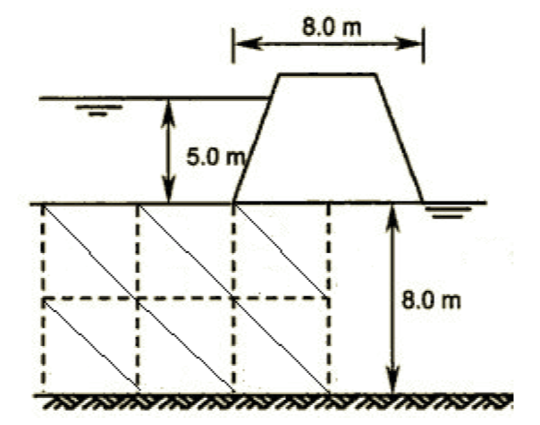
\includegraphics[width=0.65\linewidth]{principal}	
	\label{patton}	
\end{figure}


\newpage

\section*{Solução}

\vspace{10mm}



A camada de argila do problema foi discretizando em 4 elementos lineares quadráticos , como pode ser observado na seguinte figura.

\begin{figure}[H]
	\centering
	\caption{Vista global da coluna com 3 elementos}	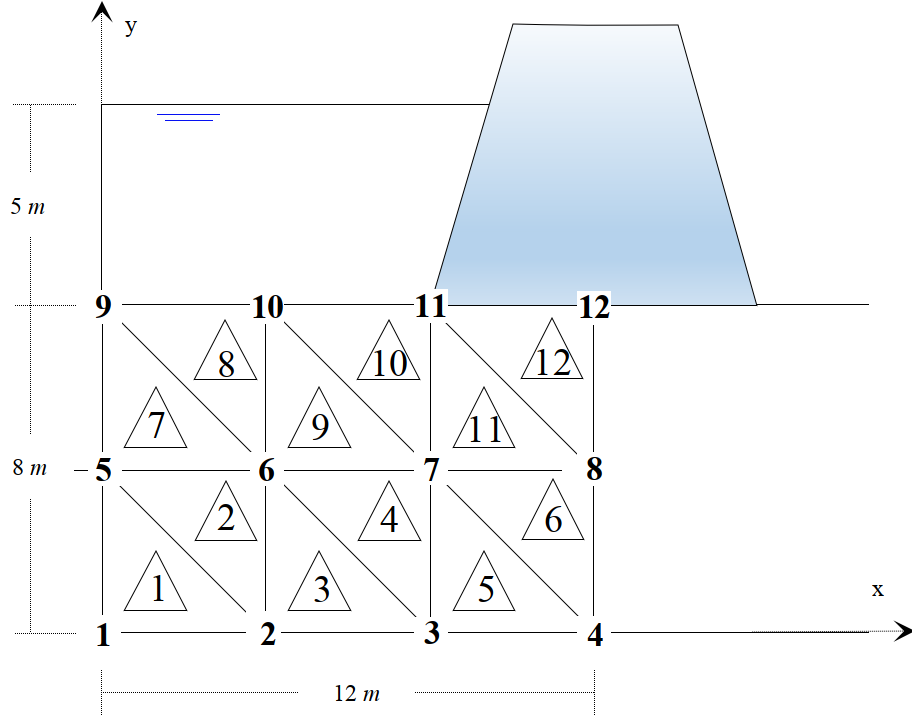
\includegraphics[width=1\linewidth]{elemento}	
	\label{elemento}	
\end{figure}

\underline{\large \textit{Método das diferenças finitas centrais}}\\


\begin{itemize}
	\item Formulação variacional	
\end{itemize}

Na seguinte equação  é mostrada a formulação variacional.
\begin{equation}
\Omega=\int_{V}\left[\frac{1}{2}c_v\left(\frac{\partial u_e}{\partial z}\right)^2+\frac{\partial u_e}{\partial t}u_e\right]dV-\int_{z_1}^{z_2}\bar{p}u_edz
\end{equation}

onde o escesso de pressão neutra \(u_e\) depende da matriz das funções de interpolação \([N]\) (elementos quadráticos) e o vetor \([q]\).
\begin{equation}
u_e=[N][q]
\end{equation}


\begin{equation}
[q]=\begin{bmatrix}
u_e^1\\u_e^2\\u_e^3
\end{bmatrix}
\end{equation}

\begin{equation}
[N]=\begin{bmatrix}
N_1&N_2&N_3
\end{bmatrix}=\begin{bmatrix}
\frac{1}{2}\xi(\xi-1)&\frac{1}{2}\xi(\xi+1)&(1-\xi^2)
\end{bmatrix}
\end{equation}

Logo, a derivada do excesso de pressão neutra respeito à profundidade é mostrada a continuação.
\begin{equation*}
\frac{\partial u_e}{\partial z}=\frac{\partial}{\partial z}[N][q]
\end{equation*}

\begin{equation*}
\frac{\partial u_e}{\partial z}=\frac{\partial}{\partial \xi}\begin{bmatrix}
\frac{1}{2}\xi(\xi-1)&\frac{1}{2}\xi(\xi+1)&(1-\xi^2)
\end{bmatrix}\cdot \frac{\partial \xi}{\partial z}\cdot[q]
\end{equation*}

\begin{equation}
\frac{\partial u_e}{\partial z}=\frac{1}{L}\begin{bmatrix}
2\xi-1&2\xi+1&-4\xi
\end{bmatrix}[q]
\end{equation}
 sendo a matriz \([B]\):
\begin{equation}
[B]=\frac{1}{L}\begin{bmatrix}
2\xi-1&2\xi+1&-4\xi
\end{bmatrix}
\end{equation}

Além, a derivada do excesso de pressão neutra respeito ao tempo é expressada na equação \ref{tempo}.

\begin{equation*}
\frac{\partial u_e}{\partial t}=\frac{\partial}{\partial t}[N][q]
\end{equation*}


\begin{equation}\label{tempo}
\frac{\partial u_e}{\partial t}=[N][\dot{q}]
\end{equation}

\begin{equation}
[\dot{q}]=\begin{bmatrix}
\dot{u_e^1}\\\dot{u_e^2}\\\dot{u_e^3}
\end{bmatrix}
\end{equation}

Ao reemplazar os valores de \(\frac{\partial u_e}{\partial z}\) e \(\frac{\partial u_e}{\partial t}\) e obtida a seguinte equação.
\begin{equation}
\Omega=\frac{A}{2}\int_{-1}^{+1}[q]^T[B]^T[R][B][q]\cdot\frac{L}{2}\cdot d\xi+A\int_{-1}^{+1}[q]^T[N]^T[N][\dot{q}]\cdot\frac{L}{2}\cdot d\xi-\int_{-1}^{+1}[q]^T[N]^T\cdot \bar{p}\cdot\frac{L}{2}\cdot d\xi
\end{equation}
\begin{equation}\label{der}
\frac{\partial \Omega}{\partial [q]}=0=\left[\frac{AL}{2}\int_{-1}^{+1}[B]^T[R][B]d\xi\right][q]+\left[\frac{AL}{2}\int_{-1}^{+1}[N]^T[N]d\xi\right][\dot{q}]=\frac{\bar{p}L}{2}\int_{-1}^{+1}[N]^Td\xi
\end{equation}
Agrupando.
\begin{equation}
[k'][q]+[k^*][\bar{p}]=[Q']
\end{equation}


\begin{itemize}
	\item Matriz elemental \([k']\)	
\end{itemize}


A matriz \([k']\) depende de \([R]=c_v\).
\begin{equation*}
[k']=\frac{L}{2}\int_{-1}^{+1}[B]^T[R][B]d\xi
\end{equation*}

\begin{equation*}
[k']=\frac{c_v}{2L}\int_{-1}^{+1}\begin{bmatrix}
2\xi-1\\2\xi+1\\-4\xi
\end{bmatrix}\begin{bmatrix}
2\xi-1&2\xi+1&-4\xi
\end{bmatrix}d\xi
\end{equation*}



\begin{equation*}\label{}
[k']=\frac{c_v}{2L} \int_{+1}^{-1}\begin{bmatrix}
4\xi^2-4\xi+1&4\xi^2-1&-8\xi^2+4\xi\\
4\xi^2-1&4\xi^2+4\xi+1&-8\xi^2-4\xi\\
-8\xi^2+4\xi&-8\xi^2-4\xi&16\xi^2
\end{bmatrix}d\xi
\end{equation*}

\begin{equation*}\label{}
[k']= \frac{c_v}{2L}\begin{bmatrix}
4\xi^3/3-2\xi^2+\xi&4\xi^3/3-\xi&-8\xi^3/3+2\xi^2\\
4\xi^3/3-\xi&4\xi^3/3+2\xi^2+\xi&-8\xi^3/3-2\xi^2\\
-8\xi^3/3+2\xi^2&-8\xi^3/3-2\xi^2&16\xi^3/3
\end{bmatrix}\biggr|_{-1}^{+1}
\end{equation*}
\begin{equation}\label{}
[k']= \frac{c_v}{6L}\begin{bmatrix}
14 &2&-16 \\
2&14&-16\\
-16&-16&32
\end{bmatrix}=\frac{c_v}{2L}[A]
\end{equation}

\begin{itemize}
	\item Matriz elemental \([k^*]\)	
\end{itemize}


A matriz \([k^*]\) de acordo a equação \ref{der} e a seguinte.
\begin{equation*}
[k^*]=\frac{L}{2}\int_{-1}^{+1}[N]^T[N]d\xi
\end{equation*}

\begin{equation*}
[k^*]=\frac{L}{2}\int_{-1}^{+1}\begin{bmatrix}
\frac{1}{2}\xi(\xi-1)\\\frac{1}{2}\xi(\xi+1)\\(1-\xi^2)
\end{bmatrix}\begin{bmatrix}
\frac{1}{2}\xi(\xi-1)&\frac{1}{2}\xi(\xi+1)&(1-\xi^2)
\end{bmatrix}d\xi
\end{equation*}

\begin{equation*}
[k^*]=\frac{L}{2}\int_{-1}^{+1}\begin{bmatrix}
\frac{\xi^4}{4}-\frac{\xi^3}{2}+\frac{\xi^2}{4}&\frac{\xi^4}{4}-\frac{\xi^2}{4}&-\frac{\xi^4}{2}+\frac{\xi^3}{2}+\frac{\xi^2}{2}-\frac{\xi}{2}\\
\frac{\xi^4}{4}-\frac{\xi^2}{4}&\frac{\xi^4}{4}+\frac{\xi^3}{2}+\frac{\xi^2}{4}&-\frac{\xi^4}{2}-\frac{\xi^3}{2}+\frac{\xi^2}{2}+\frac{\xi}{2}\\
-\frac{\xi^4}{2}+\frac{\xi^3}{2}+\frac{\xi^2}{2}-\frac{\xi}{2}&-\frac{\xi^4}{2}-\frac{\xi^3}{2}+\frac{\xi^2}{2}+\frac{\xi}{2}&\xi^4-2\xi^2+1
\end{bmatrix}d\xi
\end{equation*}

\begin{equation*}
[k^*]=\frac{L}{2}\begin{bmatrix}
\frac{\xi^5}{20}-\frac{\xi^4}{8}+\frac{\xi^3}{12}&\frac{\xi^5}{20}-\frac{\xi^3}{12}&-\frac{\xi^5}{10}+\frac{\xi^4}{8}+\frac{\xi^3}{6}-\frac{\xi^2}{4}\\
\frac{\xi^5}{20}-\frac{\xi^3}{12}&\frac{\xi^5}{20}+\frac{\xi^4}{8}+\frac{\xi^3}{12}&-\frac{\xi^5}{10}-\frac{\xi^4}{8}+\frac{\xi^3}{6}+\frac{\xi^2}{4}\\
-\frac{\xi^5}{10}+\frac{\xi^4}{8}+\frac{\xi^3}{6}-\frac{\xi^2}{4}&-\frac{\xi^5}{10}-\frac{\xi^4}{8}+\frac{\xi^3}{6}+\frac{\xi^2}{4}&\frac{\xi^5}{5}-\frac{2\xi^3}{3}+\xi
\end{bmatrix}\biggr|_{-1}^{+1}
\end{equation*}


\begin{equation}
[k^*]=\frac{L}{30}\begin{bmatrix}
4&-1&2\\
-1&4&2\\
2&2&16
\end{bmatrix}=\frac{L}{30}[B]
\end{equation}

\begin{itemize}
	\item Vetor elemental \([Q']\)	
\end{itemize}


Logo, a matriz \([Q']\) de acordo a equação \ref{der} e a seguinte.
\begin{equation*}
[{Q}']=\frac{\bar{p}L}{2}\int_{-1}^{+1}[N]^Td\xi
\end{equation*}

\begin{equation*}
[{Q}']=\frac{\bar{p}L}{2}\int_{-1}^{+1}\begin{bmatrix}
\frac{1}{2}\xi(\xi-1)\\\frac{1}{2}\xi(\xi+1)\\(1-\xi^2)
\end{bmatrix}d\xi
\end{equation*}

\begin{equation*}
[{Q}']=\frac{\bar{p}L}{4}\begin{bmatrix}
\frac{\xi^3}{3}-\frac{\xi^2}{2}\\\frac{\xi^3}{3}+\frac{\xi^2}{2}\\2\xi-\frac{2\xi^3}{3}
\end{bmatrix}\biggr|_{-1}^{+1}
\end{equation*}

\begin{equation}
[{Q}']=\frac{\bar{p}L}{12}\begin{bmatrix}
2\\2\\8
\end{bmatrix}=\frac{\bar{p}L}{12}[C]
\end{equation}

\begin{itemize}
	\item Discretização temporal no dominio do tempo - Diferença finita central
\end{itemize}

Considerando o método das diferenças centrais (\(\theta=1/2\)) temos a seguinte formulação.


\begin{equation}
\left([k^*]+\frac{\triangle t}{2}[{k}']\right)[q]_{(t)}=\left([k^*]-\frac{\triangle t}{2}[{k}']\right)[q]_{(t-\triangle t)}+\frac{\triangle t}{2}\left([{Q}']_{(t-\triangle t)}+[{Q}']_{(t)}\right)
\end{equation}

Ao reemplazar os valores correspondentes e dividir entre  \(L\), temos:

\begin{equation*}
\left(\frac{1}{30}[B]+\frac{c_v\triangle t}{12L^2}[A]\right)[q]_{(t)}=\left(\frac{1}{30}[B]+\frac{c_v\triangle t}{12L^2}[A]\right)[q]_{(t-\triangle t)}+\frac{\triangle t}{2}\left(\frac{\bar{p}L}{12}[C]_{(t-\triangle t)}+\frac{\bar{p}L}{12}[C]_{(t)}\right)
\end{equation*}

Para o presente problema o valor da pressão neutra prescrita equivale a zero \(\dot{p}=0\) e reemplazando o fator tempo na equação, temos:
\begin{equation}\label{kqQ}
\left(\frac{1}{30}[B]+\frac{\triangle T}{12}[A]\right)[q]_{(t)}=\left(\frac{1}{30}[B]+\frac{\triangle T}{12}[A]\right)[q]_{(t-\triangle t)}
\end{equation}
onde a equação \ref{kqQ} tem a forma da seguinte equação.
\begin{equation}
[k][q]_{t}=[Q]
\end{equation}

\begin{itemize}
	\item Matriz local \([k]\)	
\end{itemize}

\begin{equation}
[k]=\frac{1}{30}\begin{bmatrix}
4&-1&2\\
-1&4&2\\
2&2&16
\end{bmatrix}+\frac{\triangle T}{12}\begin{bmatrix}
14 &2&-16 \\
2&14&-16\\
-16&-16&32
\end{bmatrix}
\end{equation}
\begin{itemize}
	\item Vetor local \([Q]\)	
\end{itemize}

\begin{equation*}
[Q]=\left[\frac{1}{30}\begin{bmatrix}
4&-1&2\\
-1&4&2\\
2&2&16
\end{bmatrix}+\frac{\triangle T}{12}\begin{bmatrix}
14 &2&-16 \\
2&14&-16\\
-16&-16&32
\end{bmatrix}\right][q]_{(t-\triangle t)}
\end{equation*}


\begin{equation}
+\frac{\triangle t}{2}\left[\frac{\bar{p}L}{12}\begin{bmatrix}
2\\2\\8
\end{bmatrix}_{(t-\triangle t)}+\frac{\bar{p}L}{12}\begin{bmatrix}
2\\2\\8
\end{bmatrix}_{(t)}\right]
\end{equation}






\begin{itemize}
	\item Condições de contorno
\end{itemize}


\begin{equation}
u_e(0,t)=0;\hspace{10pt}t>0
\end{equation}

\begin{equation}
u_e(2,t)=0;\hspace{10pt}t>0
\end{equation}


\begin{itemize}
	\item Condição inicial
\end{itemize}


\begin{equation}
u_e(z,t)=100kPa;\hspace{10pt}0\leq z\leq2
\end{equation}


\begin{itemize}
	\item Matriz de correspondencia Global-local
\end{itemize}



\begin{table}[H]
	\centering
	\begin{tabular}{@{}ccccc@{}}
		\toprule
		\multirow{2}{*}{Global} & \multicolumn{4}{c}{Local} \\ \cmidrule(l){2-5} 
		& $\trinum{1}$& $\trinum{2}$ & $\trinum{3}$ & $\trinum{4}$ \\ \midrule
		1 & 1 & - & - & - \\
		2 & 3 & - & - & - \\
		3 & 2 & 1 & - & - \\
		4 & - & 3 & - & - \\
		5 & - & 2 & 1 & - \\
		6 & - & - & 3 & - \\
		7 & - & - & 2 & 1 \\
		8 & - & - & - & 3 \\
		9 & - & - & - & 2 \\ \bottomrule
	\end{tabular}
\end{table}



\begin{itemize}
	\item Montagem da matriz global
\end{itemize}
\begin{equation*}
\left[\frac{1}{30}\begin{bmatrix}
4&2 & -1& 0& 0& 0& 0& 0& 0\\
2& 16& 2& 0& 0& 0& 0& 0& 0\\
-1&2&8&2& -1& 0& 0& 0& 0\\
0&0& 2&16& 2& 0& 0& 0& 0\\
0&0&-1& 2& 8&2&-1& 0& 0\\
0&0&0&0& 2&16&2& 0& 0\\
0&0&0&0&-1&2&8&2&-1\\
0&0&0&0&0&0&2&16&2\\
0&0&0&0&0&0&-1&2&4
\end{bmatrix}\color{white}\right]\color{black}
\end{equation*}

\begin{equation*}
\color{white}\left[\color{black}+\frac{\triangle T}{12}\begin{bmatrix}
14&-16 & 2& 0& 0& 0& 0& 0& 0\\
-16& 32& -16& 0& 0& 0& 0& 0& 0\\
2&-16&28&-16& 2& 0& 0& 0& 0\\
0&0& -16&32& -16& 0& 0& 0& 0\\
0&0&2&-16& 28&-16&2& 0& 0\\
0&0&0&0& -16&32&-16& 0& 0\\
0&0&0&0&2&-16&28&-16&2\\
0&0&0&0&0&0&-16&32&-16\\
0&0&0&0&0&0&2&-16&14
\end{bmatrix}\right]\color{black}\begin{bmatrix}
u_e^1\\
u_e^2\\
u_e^3\\
u_e^4\\
u_e^5\\
u_e^6\\
u_e^7\\
u_e^8\\
u_e^9
\end{bmatrix}_{(t)}
\end{equation*}


\begin{equation*}
=\left[\frac{1}{30}\begin{bmatrix}
4&2 & -1& 0& 0& 0& 0& 0& 0\\
2& 16& 2& 0& 0& 0& 0& 0& 0\\
-1&2&8&2& -1& 0& 0& 0& 0\\
0&0& 2&16& 2& 0& 0& 0& 0\\
0&0&-1& 2& 8&2&-1& 0& 0\\
0&0&0&0& 2&16&2& 0& 0\\
0&0&0&0&-1&2&8&2&-1\\
0&0&0&0&0&0&2&16&2\\
0&0&0&0&0&0&-1&2&4
\end{bmatrix}\color{white}\right]\color{black}
\end{equation*}

\begin{equation*}
\color{white}\left[\color{black}-\frac{\triangle T}{12}\begin{bmatrix}
14&-16 & 2& 0& 0& 0& 0& 0& 0\\
-16& 32& -16& 0& 0& 0& 0& 0& 0\\
2&-16&28&-16& 2& 0& 0& 0& 0\\
0&0& -16&32& -16& 0& 0& 0& 0\\
0&0&2&-16& 28&-16&2& 0& 0\\
0&0&0&0& -16&32&-16& 0& 0\\
0&0&0&0&2&-16&28&-16&2\\
0&0&0&0&0&0&-16&32&-16\\
0&0&0&0&0&0&2&-16&14
\end{bmatrix}\right]\color{black}\begin{bmatrix}
u_e^1\\
u_e^2\\
u_e^3\\
u_e^4\\
u_e^5\\
u_e^6\\
u_e^7\\
u_e^8\\
u_e^9
\end{bmatrix}_{(t-\triangle t)}
\end{equation*}



\indent Neste problema serão considerado 10 intervalos de tempo com um \(\triangle t=1,85\) días, o que significa variações de fatores tempo iguais a \(\triangle T=1998/3125\).\\
\\
\indent Por tanto a matriz global ficaria da seguinte forma.

\begin{equation*}
\frac{10^{-5}}{3}\begin{bmatrix}
263776&-235744&21968&0&0&0&0&0&0\\
-235744&671488& -235744& 0& 0& 0& 0& 0& 0\\
21968&-235744&527552&-235744&21968& 0& 0& 0& 0\\
0&0&-235744&671488&-235744& 0& 0& 0& 0\\
0&0&21968&-235744&527552&-235744&21968& 0& 0\\
0&0&0&0& -235744&671488&-235744& 0& 0\\
0&0&0&0&21968&-235744&527552&-235744&21968\\
0&0&0&0&0&0&-235744&671488&-235744\\
0&0&0&0&0&0&21968&-235744&263776
\end{bmatrix}\begin{bmatrix}
u_1^1\\
u_e^2\\
u_e^3\\
u_e^4\\
u_e^5\\
u_e^6\\
u_e^7\\
u_e^8\\
u_e^9
\end{bmatrix}_{(t)}
\end{equation*}

\begin{equation*}
=\frac{10^{-5}}{3}\begin{bmatrix}
-183776&275744&-41968&0&0&0&0&0&0\\
275744&-351488&275744& 0& 0& 0& 0& 0& 0\\
-41968&275744&-367552&275744&-41968& 0& 0& 0& 0\\
0&0&275744&-351488&275744& 0& 0& 0& 0\\
0&0&-41968&275744&-367552&275744&-41968& 0& 0\\
0&0&0&0&275744&-351488&275744& 0& 0\\
0&0&0&0&-41968&275744&-367552&275744&-41968\\
0&0&0&0&0&0&275744&-351488&275744\\
0&0&0&0&0&0&-41968&275744&-183776
\end{bmatrix}\begin{bmatrix}
u_1^1\\
u_e^2\\
u_e^3\\
u_e^4\\
u_e^5\\
u_e^6\\
u_e^7\\
u_e^8\\
u_e^9
\end{bmatrix}_{(t-\triangle t)}
\end{equation*}
\begin{itemize}
	\item Paso 1 : \(t_1=t_0+\triangle t=1,85\) días,
\end{itemize}

No tempo \(t=0\) temos: \(u_e^1=u_e^2=u_e^3=u_e^4=u_e^5=u_e^6=u_e^7=u_e^8=100kPa\)\\
\\
\indent Além disso, o valor de (\(u_e^1=0\)).\\

\begin{equation*}
\begin{bmatrix}
671488& -235744& 0& 0& 0& 0& 0& 0\\
-235744&527552&-235744&21968& 0& 0& 0& 0\\
0&-235744&671488&-235744& 0& 0& 0& 0\\
0&21968&-235744&527552&-235744&21968& 0& 0\\
0&0&0& -235744&671488&-235744& 0& 0\\
0&0&0&21968&-235744&527552&-235744&21968\\
0&0&0&0&0&-235744&671488&-235744\\
0&0&0&0&0&21968&-235744&263776
\end{bmatrix}\begin{bmatrix}
u_e^2\\
u_e^3\\
u_e^4\\
u_e^5\\
u_e^6\\
u_e^7\\
u_e^8\\
u_e^9
\end{bmatrix}_{(t=t_1)}
=10^6\begin{bmatrix}
20\\
10\\
20\\
10\\
20\\
10\\
20\\
5
\end{bmatrix}
\end{equation*}
\indent Ao resolver a matriz com o MatLab forem obtidos os escessos de pressão neutra nodais, os quais são mostrados no seguinte vetor.
\begin{equation}\label{t1}
\begin{bmatrix}
u_e^1\\
u_e^2\\
u_e^3\\
u_e^4\\
u_e^5\\
u_e^6\\
u_e^7\\
u_e^8\\
u_e^9
\end{bmatrix}_{t=t_1=1,85dias}=\begin{bmatrix}
0\\
58,8200\\
82,7037\\
92,8765\\
97,0059\\
98,7617\\
99,4671\\
99,7501\\
99,8210
\end{bmatrix}kPa
\end{equation}

\begin{itemize}
	\item Paso 2 : \(t_2=t_1+\triangle t=3,7\) días,
\end{itemize}

Os excessos de pressão neutra do tempo \(t=t_1\) forem calculados no paso 1, ver equação \ref{t1}.\\
\\
\indent Além disso, o valor de (\(u_e^1=0\)).\\

\begin{equation*}
\begin{bmatrix}
671488& -235744& 0& 0& 0& 0& 0& 0\\
-235744&527552&-235744&21968& 0& 0& 0& 0\\
0&-235744&671488&-235744& 0& 0& 0& 0\\
0&21968&-235744&527552&-235744&21968& 0& 0\\
0&0&0& -235744&671488&-235744& 0& 0\\
0&0&0&21968&-235744&527552&-235744&21968\\
0&0&0&0&0&-235744&671488&-235744\\
0&0&0&0&0&21968&-235744&263776
\end{bmatrix}\begin{bmatrix}
u_e^2\\
u_e^3\\
u_e^4\\
u_e^5\\
u_e^6\\
u_e^7\\
u_e^8\\
u_e^9
\end{bmatrix}_{(t=t_2)}
=\begin{bmatrix}
2130525\\
7360346\\
16908869\\
9543027\\
19462699\\
9918675\\
19891535\\
4986352
\end{bmatrix}
\end{equation*}
\indent Ao resolver a matriz com o MatLab forem obtidos os escessos de pressão neutra nodais, os quais são mostrados no seguinte vetor.
\begin{equation}\label{t2}
\begin{bmatrix}
u_e^1\\
u_e^2\\
u_e^3\\
u_e^4\\
u_e^5\\
u_e^6\\
u_e^7\\
u_e^8\\
u_e^9
\end{bmatrix}_{t=t_2=3,7dias}=\begin{bmatrix}
0,0000\\
21,9125\\
53,3776\\
74,4070\\
86,8361\\
93,4213\\
96,7046\\
98,1926\\
98,6074
\end{bmatrix}kPa
\end{equation}


\begin{itemize}
	\item Paso 3 : \(t_3=t_2+\triangle t=5,55\) días,
\end{itemize}

Os excessos de pressão neutra do tempo \(t=t_2\) forem calculados no paso 2, ver equação \ref{t2}.\\
\\
\indent Além disso, o valor de (\(u_e^1=0\)).\\

\begin{equation*}
\begin{bmatrix}
671488& -235744& 0& 0& 0& 0& 0& 0\\
-235744&527552&-235744&21968& 0& 0& 0& 0\\
0&-235744&671488&-235744& 0& 0& 0& 0\\
0&21968&-235744&527552&-235744&21968& 0& 0\\
0&0&0& -235744&671488&-235744& 0& 0\\
0&0&0&21968&-235744&527552&-235744&21968\\
0&0&0&0&0&-235744&671488&-235744\\
0&0&0&0&0&21968&-235744&263776
\end{bmatrix}\begin{bmatrix}
u_e^2\\
u_e^3\\
u_e^4\\
u_e^5\\
u_e^6\\
u_e^7\\
u_e^8\\
u_e^9
\end{bmatrix}_{(t=t_3)}
=\begin{bmatrix}
7016572\\
3296143\\
12509919\\
8062215\\
17773781\\
9509721\\
19342592\\
4895848
\end{bmatrix}
\end{equation*}
\indent Ao resolver a matriz com o MatLab forem obtidos os escessos de pressão neutra nodais, os quais são mostrados no seguinte vetor.
\begin{equation}\label{t3}
\begin{bmatrix}
u_e^1\\
u_e^2\\
u_e^3\\
u_e^4\\
u_e^5\\
u_e^6\\
u_e^7\\
u_e^8\\
u_e^9
\end{bmatrix}_{t=t_3=5,55dias}=\begin{bmatrix}
0,0000\\
24,6352\\
40,4067\\
58,6676\\
73,6350\\
84,1212\\
90,5796\\
93,9532\\
94,9855
\end{bmatrix}kPa
\end{equation}


\begin{itemize}
	\item Paso 4 : \(t_4=t_3+\triangle t=7,4\) días,
\end{itemize}

Os excessos de pressão neutra do tempo \(t=t_3\) forem calculados no paso 3, ver equação \ref{t3}.\\
\\
\indent Além disso, o valor de (\(u_e^1=0\)).\\

\begin{equation*}
\begin{bmatrix}
671488& -235744& 0& 0& 0& 0& 0& 0\\
-235744&527552&-235744&21968& 0& 0& 0& 0\\
0&-235744&671488&-235744& 0& 0& 0& 0\\
0&21968&-235744&527552&-235744&21968& 0& 0\\
0&0&0& -235744&671488&-235744& 0& 0\\
0&0&0&21968&-235744&527552&-235744&21968\\
0&0&0&0&0&-235744&671488&-235744\\
0&0&0&0&0&21968&-235744&263776
\end{bmatrix}\begin{bmatrix}
u_e^2\\
u_e^3\\
u_e^4\\
u_e^5\\
u_e^6\\
u_e^7\\
u_e^8\\
u_e^9
\end{bmatrix}_{(t=t_4)}
=\begin{bmatrix}
2482928\\
5028370\\
10825357\\
6811230\\
15713598\\
8733569\\
18145041\\
4649531
\end{bmatrix}
\end{equation*}
\indent Ao resolver a matriz com o MatLab forem obtidos os escessos de pressão neutra nodais, os quais são mostrados no seguinte vetor.
\begin{equation}\label{t4}
\begin{bmatrix}
u_e^1\\
u_e^2\\
u_e^3\\
u_e^4\\
u_e^5\\
u_e^6\\
u_e^7\\
u_e^8\\
u_e^9
\end{bmatrix}_{t=t_4=7,4dias}=\begin{bmatrix}
0,0000\\
16,9236\\
37,6726\\
52,0867\\
64,7700\\
75,1837\\
82,7261\\
87,1934\\
88,6643
\end{bmatrix}kPa
\end{equation}


\begin{itemize}
	\item Paso 5 : \(t_5=t_4+\triangle t=9,25\) días,
\end{itemize}

Os excessos de pressão neutra do tempo \(t=t_4\) forem calculados no paso 4, ver equação \ref{t4}.\\
\\
\indent Além disso, o valor de (\(u_e^1=0\)).\\

\begin{equation*}
\begin{bmatrix}
671488& -235744& 0& 0& 0& 0& 0& 0\\
-235744&527552&-235744&21968& 0& 0& 0& 0\\
0&-235744&671488&-235744& 0& 0& 0& 0\\
0&21968&-235744&527552&-235744&21968& 0& 0\\
0&0&0& -235744&671488&-235744& 0& 0\\
0&0&0&21968&-235744&527552&-235744&21968\\
0&0&0&0&0&-235744&671488&-235744\\
0&0&0&0&0&21968&-235744&263776
\end{bmatrix}\begin{bmatrix}
u_e^2\\
u_e^3\\
u_e^4\\
u_e^5\\
u_e^6\\
u_e^7\\
u_e^8\\
u_e^9
\end{bmatrix}_{(t=t_5)}
=\begin{bmatrix}
4439551\\
2464269\\
9940082\\
6234813\\
14244996\\
7929037\\
16612441\\
4276838
\end{bmatrix}
\end{equation*}
\indent Ao resolver a matriz com o MatLab forem obtidos os esxessos de pressão neutra nodais, os quais são mostrados no seguinte vetor.
\begin{equation}\label{t5}
\begin{bmatrix}
u_e^1\\
u_e^2\\
u_e^3\\
u_e^4\\
u_e^5\\
u_e^6\\
u_e^7\\
u_e^8\\
u_e^9
\end{bmatrix}_{t=t_5=9,25dias}=\begin{bmatrix}
0,0000\\
17,343\\
30,5674\\
46,0547\\
58,4491\\
68,1584\\
75,2661\\
79,6459\\
81,1273
\end{bmatrix}kPa
\end{equation}




\begin{itemize}
	\item Paso 6 : \(t_6=t_5+\triangle t=11,1\) días,
\end{itemize}

Os excessos de pressão neutra do tempo \(t=t_5\) forem calculados no paso 5, ver equação \ref{t5}.\\
\\
\indent Além disso, o valor de (\(u_e^1=0\)).\\

\begin{equation*}
\begin{bmatrix}
671488& -235744& 0& 0& 0& 0& 0& 0\\
-235744&527552&-235744&21968& 0& 0& 0& 0\\
0&-235744&671488&-235744& 0& 0& 0& 0\\
0&21968&-235744&527552&-235744&21968& 0& 0\\
0&0&0& -235744&671488&-235744& 0& 0\\
0&0&0&21968&-235744&527552&-235744&21968\\
0&0&0&0&0&-235744&671488&-235744\\
0&0&0&0&0&21968&-235744&263776
\end{bmatrix}\begin{bmatrix}
u_e^2\\
u_e^3\\
u_e^4\\
u_e^5\\
u_e^6\\
u_e^7\\
u_e^8\\
u_e^9
\end{bmatrix}_{(t=t_6)}
=\begin{bmatrix}
2332921\\
3793435\\
8358091\\
5568873\\
12914304\\
7234201\\
15129964\\
3893861
\end{bmatrix}
\end{equation*}
\indent Ao resolver a matriz com o MatLab forem obtidos os esxessos de pressão neutra nodais, os quais são mostrados no seguinte vetor.
\begin{equation}\label{t6}
\begin{bmatrix}
u_e^1\\
u_e^2\\
u_e^3\\
u_e^4\\
u_e^5\\
u_e^6\\
u_e^7\\
u_e^8\\
u_e^9
\end{bmatrix}_{t=t_6=11,1dias}=\begin{bmatrix}
0,0000\\
13,8868\\
29,6590\\
41,2834\\
52,4776\\
61,6662\\
68,3899\\
72,4610\\
73,8267
\end{bmatrix}kPa
\end{equation}
\begin{itemize}
	\item Paso 7 : \(t_7=t_6+\triangle t=12,95\) días,
\end{itemize}

Os excessos de pressão neutra do tempo \(t=t_6\) forem calculados no paso 6, ver equação \ref{t6}.\\
\\
\indent Além disso, o valor de (\(u_e^1=0\)).\\

\begin{equation*}
\begin{bmatrix}
671488& -235744& 0& 0& 0& 0& 0& 0\\
-235744&527552&-235744&21968& 0& 0& 0& 0\\
0&-235744&671488&-235744& 0& 0& 0& 0\\
0&21968&-235744&527552&-235744&21968& 0& 0\\
0&0&0& -235744&671488&-235744& 0& 0\\
0&0&0&21968&-235744&527552&-235744&21968\\
0&0&0&0&0&-235744&671488&-235744\\
0&0&0&0&0&21968&-235744&263776
\end{bmatrix}\begin{bmatrix}
u_e^2\\
u_e^3\\
u_e^4\\
u_e^5\\
u_e^6\\
u_e^7\\
u_e^8\\
u_e^9
\end{bmatrix}_{(t=t_7)}
=\begin{bmatrix}
3297248\\
2109247\\
8138055\\
4984571\\
11653559\\
6547187\\
13746202\\
3542923
\end{bmatrix}
\end{equation*}
\indent Ao resolver a matriz com o MatLab forem obtidos os esxessos de pressão neutra nodais, os quais são mostrados no seguinte vetor.
\begin{equation}\label{t7}
\begin{bmatrix}
u_e^1\\
u_e^2\\
u_e^3\\
u_e^4\\
u_e^5\\
u_e^6\\
u_e^7\\
u_e^8\\
u_e^9
\end{bmatrix}_{t=t_7=12,95dias}=\begin{bmatrix}
0,0000\\
13,6525\\
24,9009\\
37,5549\\
47,5490\\
55,8013\\
61,9610\\
65,7622\\
67,0448
\end{bmatrix}kPa
\end{equation}

\begin{itemize}
	\item Paso 8 : \(t_8=t_7+\triangle t=14,8\) días,
\end{itemize}

Os excessos de pressão neutra do tempo \(t=t_7\) forem calculados no paso 7, ver equação \ref{t7}.\\
\\
\indent Além disso, o valor de (\(u_e^1=0\)).\\

\begin{equation*}
\begin{bmatrix}
671488& -235744& 0& 0& 0& 0& 0& 0\\
-235744&527552&-235744&21968& 0& 0& 0& 0\\
0&-235744&671488&-235744& 0& 0& 0& 0\\
0&21968&-235744&527552&-235744&21968& 0& 0\\
0&0&0& -235744&671488&-235744& 0& 0\\
0&0&0&21968&-235744&527552&-235744&21968\\
0&0&0&0&0&-235744&671488&-235744\\
0&0&0&0&0&21968&-235744&263776
\end{bmatrix}\begin{bmatrix}
u_e^2\\
u_e^3\\
u_e^4\\
u_e^5\\
u_e^6\\
u_e^7\\
u_e^8\\
u_e^9
\end{bmatrix}_{(t=t_8)}
=\begin{bmatrix}
2719554\\
2067584\\
2972221\\
6777529\\
4620262\\
10583238\\
5937244\\
12457951\\
3211928
\end{bmatrix}
\end{equation*}
\indent Ao resolver a matriz com o MatLab forem obtidos os esxessos de pressão neutra nodais, os quais são mostrados no seguinte vetor.
\begin{equation}\label{t8}
\begin{bmatrix}
u_e^1\\
u_e^2\\
u_e^3\\
u_e^4\\
u_e^5\\
u_e^6\\
u_e^7\\
u_e^8\\
u_e^9
\end{bmatrix}_{t=t_8=14,8dias}=\begin{bmatrix}
0,0000\\
11,5120\\
24,0202\\
33,6461\\
43,0672\\
50,6056\\
56,1838\\
59,6151\\
60,7772
\end{bmatrix}kPa
\end{equation}

\begin{itemize}
	\item Paso 9 : \(t_9=t_8+\triangle t=16,65\) días,
\end{itemize}

Os excessos de pressão neutra do tempo \(t=t_8\) forem calculados no paso 8, ver equação \ref{t8}.\\
\\
\indent Além disso, o valor de (\(u_e^1=0\)).\\

\begin{equation*}
\begin{bmatrix}
671488& -235744& 0& 0& 0& 0& 0& 0\\
-235744&527552&-235744&21968& 0& 0& 0& 0\\
0&-235744&671488&-235744& 0& 0& 0& 0\\
0&21968&-235744&527552&-235744&21968& 0& 0\\
0&0&0& -235744&671488&-235744& 0& 0\\
0&0&0&21968&-235744&527552&-235744&21968\\
0&0&0&0&0&-235744&671488&-235744\\
0&0&0&0&0&21968&-235744&263776
\end{bmatrix}\begin{bmatrix}
u_e^2\\
u_e^3\\
u_e^4\\
u_e^5\\
u_e^6\\
u_e^7\\
u_e^8\\
u_e^9
\end{bmatrix}_{(t=t_9)}
=\begin{bmatrix}
2577096\\
1815958\\
6672748\\
4036464\\
9580607\\
5384087\\
11297302\\
2911194
\end{bmatrix}
\end{equation*}
\indent Ao resolver a matriz com o MatLab forem obtidos os esxessos de pressão neutra nodais, os quais são mostrados no seguinte vetor.
\begin{equation}\label{t9}
\begin{bmatrix}
u_e^1\\
u_e^2\\
u_e^3\\
u_e^4\\
u_e^5\\
u_e^6\\
u_e^7\\
u_e^8\\
u_e^9
\end{bmatrix}_{t=t_9=16,65dias}=\begin{bmatrix}
0,0000\\
11,0420\\
20,5200\\
30,8005\\
38,9063\\
45,7982\\
50,9043\\
54,0370\\
55,0915
\end{bmatrix}kPa
\end{equation}
\begin{itemize}
	\item Paso 10 : \(t_10=t_9+\triangle t=18,5\) días,
\end{itemize}

Os excessos de pressão neutra do tempo \(t=t_9\) forem calculados no paso 9, ver equação \ref{t9}.\\
\\
\indent Além disso, o valor de (\(u_e^1=0\)).\\

\begin{equation*}
\begin{bmatrix}
671488& -235744& 0& 0& 0& 0& 0& 0\\
-235744&527552&-235744&21968& 0& 0& 0& 0\\
0&-235744&671488&-235744& 0& 0& 0& 0\\
0&21968&-235744&527552&-235744&21968& 0& 0\\
0&0&0& -235744&671488&-235744& 0& 0\\
0&0&0&21968&-235744&527552&-235744&21968\\
0&0&0&0&0&-235744&671488&-235744\\
0&0&0&0&0&21968&-235744&263776
\end{bmatrix}\begin{bmatrix}
u_e^2\\
u_e^3\\
u_e^4\\
u_e^5\\
u_e^6\\
u_e^7\\
u_e^8\\
u_e^9
\end{bmatrix}_{(t=t_10)}
=\begin{bmatrix}
1777136\\
2362832\\
5560440\\
3824009\\
8667216\\
4874080\\
10234349\\
2639531
\end{bmatrix}
\end{equation*}
\indent Ao resolver a matriz com o MatLab forem obtidos os esxessos de pressão neutra nodais, os quais são mostrados no seguinte vetor.
\begin{equation}\label{t10}
\begin{bmatrix}
u_e^1\\
u_e^2\\
u_e^3\\
u_e^4\\
u_e^5\\
u_e^6\\
u_e^7\\
u_e^8\\
u_e^9
\end{bmatrix}_{t=t_{10}=18,5dias}=\begin{bmatrix}
0,0000\\
9,5229\\
19,5865\\
27,5835\\
35,3950\\
41,5259\\
46,1213\\
48,9601\\
49,9226
\end{bmatrix}kPa
\end{equation}

\begin{itemize}
	\item Resumen
\end{itemize}

O resumen dos resultados das pressões neutras nódais \((u_e)\) são nostradas na seguinte tabela e a Fig. \ref{result}.

\begin{table}[H]
		\caption{Excesso de pressão neutra nodai \((u_e)\) respeito do tempo}
	\begin{tabular}{@{}ccccccccccc@{}}
		\toprule
		\multirow{2}{*}{\begin{tabular}[c]{@{}c@{}} Nós\end{tabular}} & \multicolumn{10}{c}{t (días)} \\ \cmidrule(l){2-11} 
		& 1,85 & 3,7 & 5,55 & 7,4 & 9,25 & 11,1 & 12,95 & 14,8 & 16,65 & 18,5 \\ \midrule
		1 & 0,0000 & 0,0000 & 0,0000 & 0,0000 & 0,0000 & 0,0000 & 0,0000 & 0,0000 & 0,0000 & 0,0000 \\
		2 & 58,8200 & 21,9125 & 24,6352 & 16,9236 & 17,3430 & 13,8868 & 13,6525 & 11,5120 & 11,0420 & 9,5229 \\
		3 & 82,7037 & 53,3776 & 40,4067 & 37,6726 & 30,5674 & 29,6590 & 24,9009 & 24,0202 & 20,5200 & 19,5865 \\
		4 & 92,8765 & 74,4070 & 58,6676 & 52,0867 & 46,0547 & 41,2834 & 37,5549 & 33,6461 & 30,8005 & 27,5835 \\
		8 & 97,0059 & 86,8361 & 73,6350 & 64,7700 & 58,4491 & 52,4776 & 47,5490 & 43,0672 & 38,9063 & 35,3950 \\
		6 & 98,7617 & 93,4213 & 84,1212 & 75,1837 & 68,1584 & 61,6662 & 55,8013 & 50,6056 & 45,7982 & 41,5259 \\
		7 & 99,4671 & 96,7046 & 90,5796 & 82,7261 & 75,2661 & 68,3899 & 61,9610 & 56,1838 & 50,9043 & 46,1213 \\
		8 & 99,7501 & 98,1926 & 93,9532 & 87,1934 & 79,6459 & 72,4610 & 65,7622 & 59,6151 & 54,037 & 48,9601 \\
		9 & 99,8210 & 98,6074 & 94,9855 & 88,6643 & 81,1273 & 73,8267 & 67,0448 & 60,7772 & 55,0915 & 49,9226 \\ \bottomrule
	\end{tabular}
\end{table}

\begin{figure}[H]
	\centering
	\caption{Evolução de \(u_e\) nodais ao longo do tempo (até \(t=18,5\) días)}
	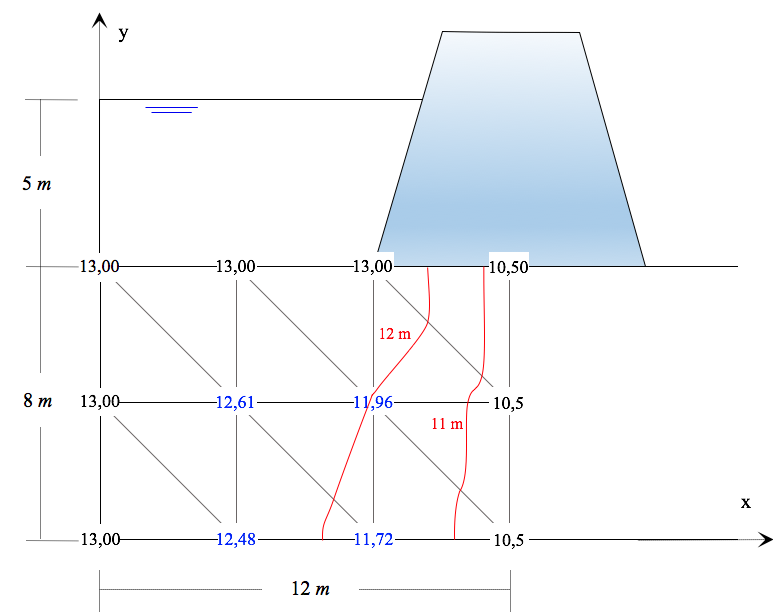
\includegraphics[width=1\linewidth]{result}	
	\label{result}	
\end{figure}
 Finalmente, uma comparação dos resultados analíticos e numéricos de excessos de pressão neutra nodais no tempo \(t=18,5\) días pode ser observada na Fig. \ref{comparacion}
\begin{figure}[H]
	\centering
	\caption{Evolução de \(u_e\) ao longo do tempo (até \(t=18,5\) días)}
	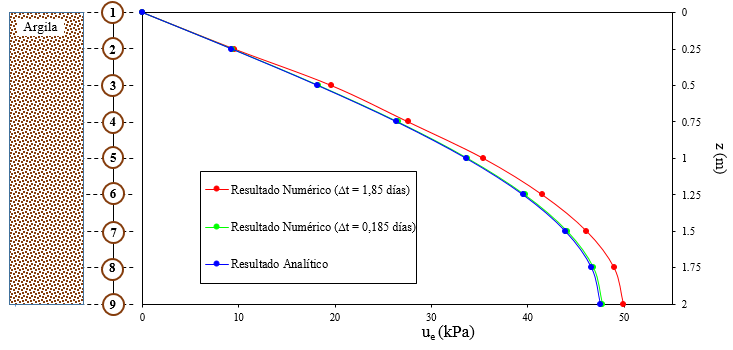
\includegraphics[width=1\linewidth]{comparacion}	
	\label{comparacion}	
\end{figure}




%BIBLIOGRAPHY
%\bibliographystyle{apalike}
%\bibliography{bibliography}


\end{document}
